\section{Desarrollo}



\subsection{Colinealidad}

\begin{figure}[H]
    \centering
    \begin{tikzpicture}[xscale = 1.5, yscale = 1.5]

\end{tikzpicture}
\end{figure}

Tres puntos son \textbf{colineales} si se encuentran sobre una misma línea.
Dicho esto, presentaremos algunos enfoques que nos ayudarán a probar que tres puntos son colineales al resolver problemas de geometría.

Hay tres formas más comunes de angulear que nos permiten probar que tres puntos $A$, $B$ y $C$ son colineales.

\begin{figure}[H]
    \centering
    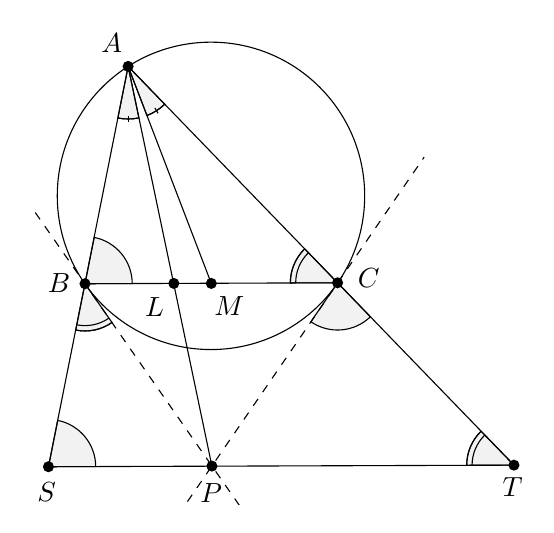
\begin{tikzpicture}[scale = 0.4]
    \clip(-2.36,-10.08) rectangle (13.47,5.06);
    \draw [shift={(-0.54,-3.07)},fill=black,fill opacity=0.05] (0,0) -- (0.2:1.5) arc (0.2:78.71:1.5) -- cycle;
    \draw [shift={(7.48,-3.04)},fill=black,fill opacity=0.05] (0,0) -- (-124.46:1.5) arc (-124.46:-45.95:1.5) -- cycle;
    \draw [shift={(-1.7,-8.88)},fill=black,fill opacity=0.05] (0,0) -- (0.2:1.5) arc (0.2:78.71:1.5) -- cycle;
    \draw [shift={(-0.54,-3.07)},fill=black,fill opacity=0.05] (0,0) -- (-101.29:1.5) arc (-101.29:-55.14:1.5) -- cycle;
    \draw [shift={(7.48,-3.04)},fill=black,fill opacity=0.05] (0,0) -- (134.05:1.5) arc (134.05:180.2:1.5) -- cycle;
    \draw [shift={(13.08,-8.83)},fill=black,fill opacity=0.05] (0,0) -- (134.05:1.5) arc (134.05:180.2:1.5) -- cycle;
    \draw [shift={(0.83,3.83)},fill=black,fill opacity=0.05] (0,0) -- (-101.29:1.67) arc (-101.29:-78.18:1.67) -- cycle;
    \draw [shift={(0.83,3.83)},fill=black,fill opacity=0.05] (0,0) -- (-69.06:1.67) arc (-69.06:-45.95:1.67) -- cycle;
    \draw(3.46,-0.28) circle (4.88cm);
    \draw (-0.54,-3.07)-- (7.48,-3.04);
    \draw (0.83,3.83)-- (-1.7,-8.88);
    \draw (0.83,3.83)-- (13.08,-8.83);
    \draw (-1.7,-8.88)-- (13.08,-8.83);
    \draw (0.83,3.83)-- (3.49,-8.86);
    \draw (0.83,3.83)-- (3.47,-3.06);
    \draw [dash pattern=on 3pt off 3pt,domain=-2.1176316762214267:13.472829432059696] plot(\x,{(-21.59-8.05*\x)/5.61});
    \draw [dash pattern=on 3pt off 3pt,domain=-2.361745286484902:10.226227746616733] plot(\x,{(--93.93-9.81*\x)/-6.74});
    \draw [shift={(-0.54,-3.07)}] (-101.29:1.5) arc (-101.29:-55.14:1.5);
    \draw [shift={(-0.54,-3.07)}] (-101.29:1.33) arc (-101.29:-55.14:1.33);
    \draw [shift={(7.48,-3.04)}] (134.05:1.5) arc (134.05:180.2:1.5);
    \draw [shift={(7.48,-3.04)}] (134.05:1.33) arc (134.05:180.2:1.33);
    \draw [shift={(13.08,-8.83)}] (134.05:1.5) arc (134.05:180.2:1.5);
    \draw [shift={(13.08,-8.83)}] (134.05:1.33) arc (134.05:180.2:1.33);
    \draw [shift={(0.83,3.83)}] (-101.29:1.67) arc (-101.29:-78.18:1.67);
    \draw(0.84,2.27) -- (0.84,2.07);
    \draw [shift={(0.83,3.83)}] (-69.06:1.67) arc (-69.06:-45.95:1.67);
    \draw(1.68,2.51) -- (1.78,2.34);
    \begin{scriptsize}
        \normalsize
        \fill [color=black] (0.83,3.83) circle (5pt);
        \draw[color=black] (0.31,4.56) node {$A$};
        \fill [color=black] (3.49,-8.86) circle (5pt);
        \draw[color=black] (3.47,-9.7) node {$P$};
        \fill [color=black] (-0.54,-3.07) circle (5pt);
        \draw[color=black] (-1.36,-3.04) node {$B$};
        \fill [color=black] (7.48,-3.04) circle (5pt);
        \draw[color=black] (8.47,-2.88) node {$C$};
        \fill [color=black] (-1.7,-8.88) circle (5pt);
        \draw[color=black] (-1.76,-9.68) node {$S$};
        \fill [color=black] (13.08,-8.83) circle (5pt);
        \draw[color=black] (13.04,-9.54) node {$T$};
        \fill [color=black] (2.28,-3.06) circle (5pt);
        \draw[color=black] (1.67,-3.81) node {$L$};
        \fill [color=black] (3.47,-3.06) circle (5pt);
        \draw[color=black] (4.04,-3.78) node {$M$};
    \end{scriptsize}
\end{tikzpicture}
    \caption{Tres configuraciones de colinealidad.}
\end{figure}

En la primera configuración\footnote{Comenzando de izquierda a derecha.}, necesitaremos dos puntos adicionales que ya son colineales con nuestro punto ``medio'' $B$.
Sean esos puntos $X$ e $Y$.
Si $\angle XBA = \angle YBC$, entonces los puntos $A$, $B$ y $C$ son colineales.

En la segunda configuración, necesitaremos un punto extra $X$ que no esté en la supuesta línea $A - B - C$.
Si $\angle ABX + \angle XBC = 180^\circ$, entonces los puntos $A$, $B$ y $C$ son colineales.

En la tercera configuración, también necesitaremos un punto extra $X$ que no esté en la supuesta línea $A - B - C$.
Si $\angle XAB = \angle XAC$, entonces los puntos $A$, $B$ y $C$ son colineales.


\begin{section-theorem.tcb}[Teorema de Menelao]
    Dado un triángulo $ABC$, sean $D$, $E$ y $F$ puntos sobre los lados (o sus prolongaciones) $BC$, $CA$ y $AB$, respectivamente.
    Entonces los puntos $D$, $E$ y $F$ son colineales si y sólo si
    \[
        \frac{CD}{BD} \cdot \frac{BF}{FA} \cdot \frac{AE}{EC} = 1.
    \]
\end{section-theorem.tcb}
\begin{proof}
    La demostración se deja como ejercicio al lector.
\end{proof}

\begin{section-theorem.tcb}[Menelao trigonométrico]
    Dado un triángulo $ABC$, sean $D$, $E$ y $F$ puntos sobre los lados (o sus prolongaciones) $BC$, $CA$ y $AB$, respectivamente.
    Entonces los puntos $D$, $E$ y $F$ son colineales si y sólo si
    \[
        \frac{\sen(\angle CAD)}{\sen(\angle BAD)} \cdot \frac{\sen(\angle BCF)}{\sen(\angle FCA)} \cdot \frac{\sen(\angle ABE)}{\sen(\angle EBC)} = 1.
    \]
\end{section-theorem.tcb}
\begin{proof}
    La demostración se deja como ejercicio al lector.
\end{proof}


\begin{section-theorem.tcb}[Recta de Gauss]
    Sean $L$ y $M$ los puntos medios de las diagonales $AC$ y $BD$ del cuadrilátero $ABCD$.
    Las rectas $AB$ y $CD$ se cortan en $E$, y las rectas $AD$ y $BC$ se cortan en $F$.
    Sea $N$ el punto medio de $EF$.
    Entonces los puntos $L$, $M$ y $N$ colineales.
\end{section-theorem.tcb}



\subsection{Teorema de Pappus}

\begin{section-theorem.tcb}[Teorema de Pappus]
    En todo hexágono (no necesariamente convexo) en el que sus vértices no consecutivos están alineados, las intersecciones de sus lados opuestos son colineales.
\end{section-theorem.tcb}




\subsection{Teorema de Desargues}
\begin{section-theorem.tcb}[Teorema de Desargues]
    Dos triángulos están en perspectiva si y solo si son coaxiales.
\end{section-theorem.tcb}

\begin{remark.tcb}
    Dos triángulos están en \textbf{perspectiva} si las rectas que unen sus vértices correspondientes son concurrentes.
\end{remark.tcb}

\begin{remark.tcb}
    Dos triángulos son \textbf{coaxiales} cuando los puntos de intersección de los lados correspondientes son colineales.
\end{remark.tcb}

\subsection{Agregados culturales y preguntas}






\section{Ejercicios y Problemas}
Sección de ejercicios y problemas para el autoestudio.